% Options for packages loaded elsewhere
% Options for packages loaded elsewhere
\PassOptionsToPackage{unicode}{hyperref}
\PassOptionsToPackage{hyphens}{url}
%
\documentclass[
  english,
  russian,
  12pt,
  a4paper,
  DIV=11,
  numbers=noendperiod]{scrreprt}
\usepackage{xcolor}
\usepackage{amsmath,amssymb}
\setcounter{secnumdepth}{5}
\usepackage{iftex}
\ifPDFTeX
  \usepackage[T1]{fontenc}
  \usepackage[utf8]{inputenc}
  \usepackage{textcomp} % provide euro and other symbols
\else % if luatex or xetex
  \usepackage{unicode-math} % this also loads fontspec
  \defaultfontfeatures{Scale=MatchLowercase}
  \defaultfontfeatures[\rmfamily]{Ligatures=TeX,Scale=1}
\fi
\usepackage{lmodern}
\ifPDFTeX\else
  % xetex/luatex font selection
\fi
% Use upquote if available, for straight quotes in verbatim environments
\IfFileExists{upquote.sty}{\usepackage{upquote}}{}
\IfFileExists{microtype.sty}{% use microtype if available
  \usepackage[]{microtype}
  \UseMicrotypeSet[protrusion]{basicmath} % disable protrusion for tt fonts
}{}
\usepackage{setspace}
% Make \paragraph and \subparagraph free-standing
\makeatletter
\ifx\paragraph\undefined\else
  \let\oldparagraph\paragraph
  \renewcommand{\paragraph}{
    \@ifstar
      \xxxParagraphStar
      \xxxParagraphNoStar
  }
  \newcommand{\xxxParagraphStar}[1]{\oldparagraph*{#1}\mbox{}}
  \newcommand{\xxxParagraphNoStar}[1]{\oldparagraph{#1}\mbox{}}
\fi
\ifx\subparagraph\undefined\else
  \let\oldsubparagraph\subparagraph
  \renewcommand{\subparagraph}{
    \@ifstar
      \xxxSubParagraphStar
      \xxxSubParagraphNoStar
  }
  \newcommand{\xxxSubParagraphStar}[1]{\oldsubparagraph*{#1}\mbox{}}
  \newcommand{\xxxSubParagraphNoStar}[1]{\oldsubparagraph{#1}\mbox{}}
\fi
\makeatother


\usepackage{longtable,booktabs,array}
\usepackage{calc} % for calculating minipage widths
% Correct order of tables after \paragraph or \subparagraph
\usepackage{etoolbox}
\makeatletter
\patchcmd\longtable{\par}{\if@noskipsec\mbox{}\fi\par}{}{}
\makeatother
% Allow footnotes in longtable head/foot
\IfFileExists{footnotehyper.sty}{\usepackage{footnotehyper}}{\usepackage{footnote}}
\makesavenoteenv{longtable}
\usepackage{graphicx}
\makeatletter
\newsavebox\pandoc@box
\newcommand*\pandocbounded[1]{% scales image to fit in text height/width
  \sbox\pandoc@box{#1}%
  \Gscale@div\@tempa{\textheight}{\dimexpr\ht\pandoc@box+\dp\pandoc@box\relax}%
  \Gscale@div\@tempb{\linewidth}{\wd\pandoc@box}%
  \ifdim\@tempb\p@<\@tempa\p@\let\@tempa\@tempb\fi% select the smaller of both
  \ifdim\@tempa\p@<\p@\scalebox{\@tempa}{\usebox\pandoc@box}%
  \else\usebox{\pandoc@box}%
  \fi%
}
% Set default figure placement to htbp
\def\fps@figure{htbp}
\makeatother



\ifLuaTeX
\usepackage[bidi=basic,provide=*]{babel}
\else
\usepackage[bidi=default,provide=*]{babel}
\fi
% get rid of language-specific shorthands (see #6817):
\let\LanguageShortHands\languageshorthands
\def\languageshorthands#1{}


\setlength{\emergencystretch}{3em} % prevent overfull lines

\providecommand{\tightlist}{%
  \setlength{\itemsep}{0pt}\setlength{\parskip}{0pt}}



 
\usepackage[style=gost-numeric,backend=biber,langhook=extras,autolang=other*]{biblatex}
\addbibresource{bib/cite.bib}

\usepackage[]{csquotes}

\KOMAoption{captions}{tableheading}
\usepackage{indentfirst}
\usepackage{float}
\floatplacement{figure}{H}
\usepackage{libertine}
\usepackage{indentfirst}
\usepackage{float}
\floatplacement{figure}{H}
\usepackage[math,RM={Scale=0.94},SS={Scale=0.94},SScon={Scale=0.94},TT={Scale=MatchLowercase,FakeStretch=0.9},DefaultFeatures={Ligatures=Common}]{plex-otf}
\makeatletter
\@ifpackageloaded{caption}{}{\usepackage{caption}}
\AtBeginDocument{%
\ifdefined\contentsname
  \renewcommand*\contentsname{Содержание}
\else
  \newcommand\contentsname{Содержание}
\fi
\ifdefined\listfigurename
  \renewcommand*\listfigurename{Список иллюстраций}
\else
  \newcommand\listfigurename{Список иллюстраций}
\fi
\ifdefined\listtablename
  \renewcommand*\listtablename{Список таблиц}
\else
  \newcommand\listtablename{Список таблиц}
\fi
\ifdefined\figurename
  \renewcommand*\figurename{Рисунок}
\else
  \newcommand\figurename{Рисунок}
\fi
\ifdefined\tablename
  \renewcommand*\tablename{Таблица}
\else
  \newcommand\tablename{Таблица}
\fi
}
\@ifpackageloaded{float}{}{\usepackage{float}}
\floatstyle{ruled}
\@ifundefined{c@chapter}{\newfloat{codelisting}{h}{lop}}{\newfloat{codelisting}{h}{lop}[chapter]}
\floatname{codelisting}{Список}
\newcommand*\listoflistings{\listof{codelisting}{Листинги}}
\makeatother
\makeatletter
\makeatother
\makeatletter
\@ifpackageloaded{caption}{}{\usepackage{caption}}
\@ifpackageloaded{subcaption}{}{\usepackage{subcaption}}
\makeatother
\usepackage{bookmark}
\IfFileExists{xurl.sty}{\usepackage{xurl}}{} % add URL line breaks if available
\urlstyle{same}
\hypersetup{
  pdftitle={Лабораторная работа №4},
  pdfauthor={Перфилов Александр Константинович \textbar{} группа НПИбд 03-24},
  pdflang={ru-RU},
  hidelinks,
  pdfcreator={LaTeX via pandoc}}


\title{Лабораторная работа №4}
\usepackage{etoolbox}
\makeatletter
\providecommand{\subtitle}[1]{% add subtitle to \maketitle
  \apptocmd{\@title}{\par {\large #1 \par}}{}{}
}
\makeatother
\subtitle{Работа с програмными пакетами}
\author{Перфилов Александр Константинович \textbar{} группа НПИбд 03-24}
\date{}
\begin{document}
\maketitle

\renewcommand*\contentsname{Содержание}
{
\setcounter{tocdepth}{1}
\tableofcontents
}
\listoffigures
\listoftables

\setstretch{1.5}
\chapter{Цель
работы}\label{ux446ux435ux43bux44c-ux440ux430ux431ux43eux442ux44b}

Получить навыки управления системными службами операционной системы
посред- ством systemd. \#\# Управление сервисами

Заходим под уч запись root

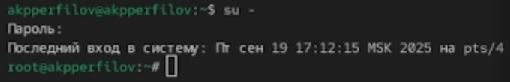
\includegraphics[width=0.71\linewidth,height=\textheight,keepaspectratio]{./home/akpperfilov/work/study/2025-2026/Основы администрирования операционных систем/os2/study_2025-2026_os2/labs/lab05/report/image/1.jpg}

Проверяем статус службы Very Secure FTP

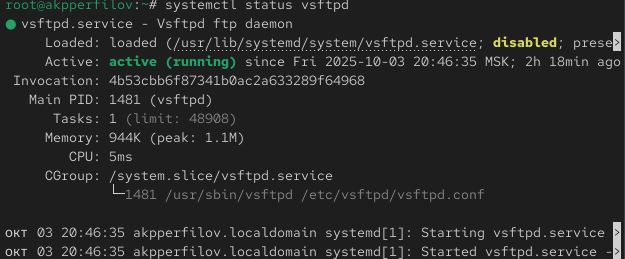
\includegraphics[width=0.71\linewidth,height=\textheight,keepaspectratio]{./home/akpperfilov/work/study/2025-2026/Основы администрирования операционных систем/os2/study_2025-2026_os2/labs/lab05/report/image/2.jpg}

Установливаем службу Very Secure FTP

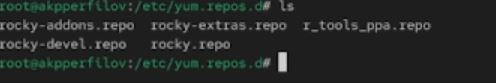
\includegraphics[width=0.71\linewidth,height=\textheight,keepaspectratio]{./home/akpperfilov/work/study/2025-2026/Основы администрирования операционных систем/os2/study_2025-2026_os2/labs/lab05/report/image/3.jpg}

Запускаем службу Very Secure FTP

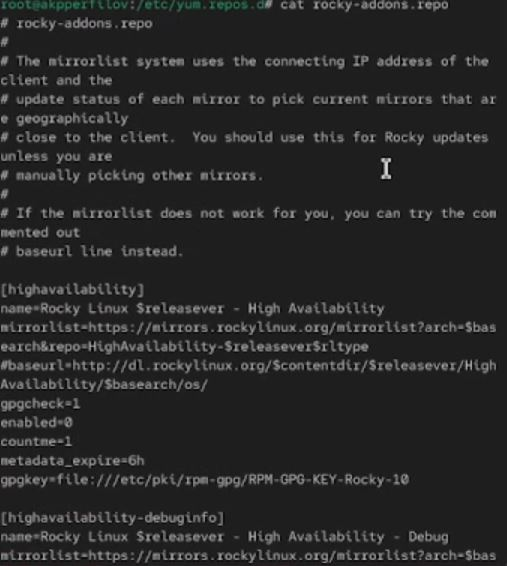
\includegraphics[width=0.71\linewidth,height=\textheight,keepaspectratio]{./home/akpperfilov/work/study/2025-2026/Основы администрирования операционных систем/os2/study_2025-2026_os2/labs/lab05/report/image/4.jpg}

Проверяем статус службы Very Secure FTP

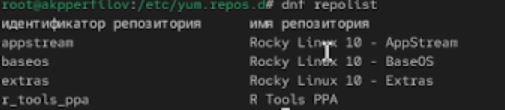
\includegraphics[width=0.71\linewidth,height=\textheight,keepaspectratio]{./home/akpperfilov/work/study/2025-2026/Основы администрирования операционных систем/os2/study_2025-2026_os2/labs/lab05/report/image/5.jpg}

Вывод команды должен показать, что служба в настоящее время работает, но
не будет активирована при перезапуске операционной системы

Добавляем службу Very Secure FTP в автозапуск при загрузке операционной
системы

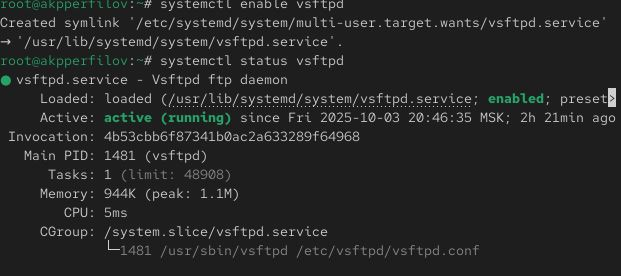
\includegraphics[width=0.71\linewidth,height=\textheight,keepaspectratio]{./home/akpperfilov/work/study/2025-2026/Основы администрирования операционных систем/os2/study_2025-2026_os2/labs/lab05/report/image/6.jpg}

Выведим на экран символические ссылки, ответственные за запуск различных
серви- сов

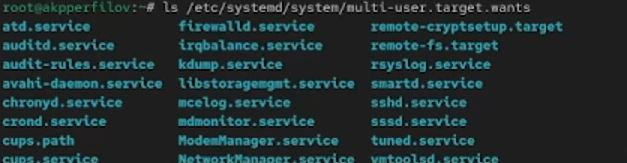
\includegraphics[width=0.71\linewidth,height=\textheight,keepaspectratio]{./home/akpperfilov/work/study/2025-2026/Основы администрирования операционных систем/os2/study_2025-2026_os2/labs/lab05/report/image/7.jpg}

Добавляем службу Very Secure FTP в автозапуск

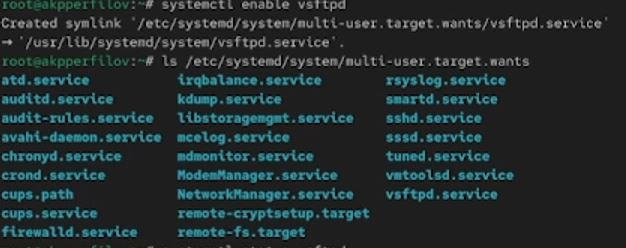
\includegraphics[width=0.71\linewidth,height=\textheight,keepaspectratio]{./home/akpperfilov/work/study/2025-2026/Основы администрирования операционных систем/os2/study_2025-2026_os2/labs/lab05/report/image/8.jpg}

Проверяем статус службы Very Secure FTP

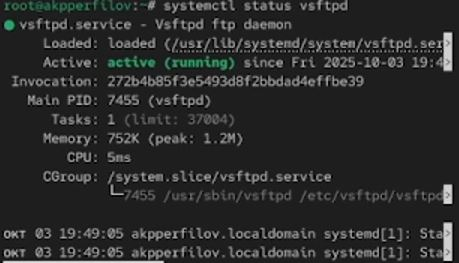
\includegraphics[width=0.71\linewidth,height=\textheight,keepaspectratio]{./home/akpperfilov/work/study/2025-2026/Основы администрирования операционных систем/os2/study_2025-2026_os2/labs/lab05/report/image/9.jpg}

Выводим на экран список зависимостей юнита

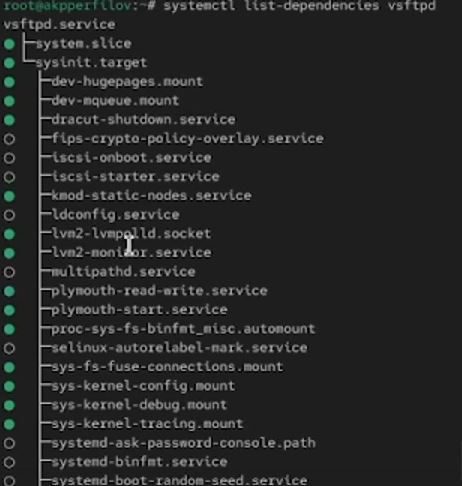
\includegraphics[width=0.71\linewidth,height=\textheight,keepaspectratio]{./home/akpperfilov/work/study/2025-2026/Основы администрирования операционных систем/os2/study_2025-2026_os2/labs/lab05/report/image/10.jpg}

Выводим на экран список юнитов, которые зависят от данного юнита

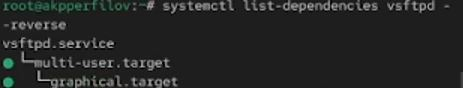
\includegraphics[width=0.71\linewidth,height=\textheight,keepaspectratio]{./home/akpperfilov/work/study/2025-2026/Основы администрирования операционных систем/os2/study_2025-2026_os2/labs/lab05/report/image/11.jpg}

\chapter{Конфликты
юнитов}\label{ux43aux43eux43dux444ux43bux438ux43aux442ux44b-ux44eux43dux438ux442ux43eux432}

Получаем полномочия администратора и устанавливаем iptables

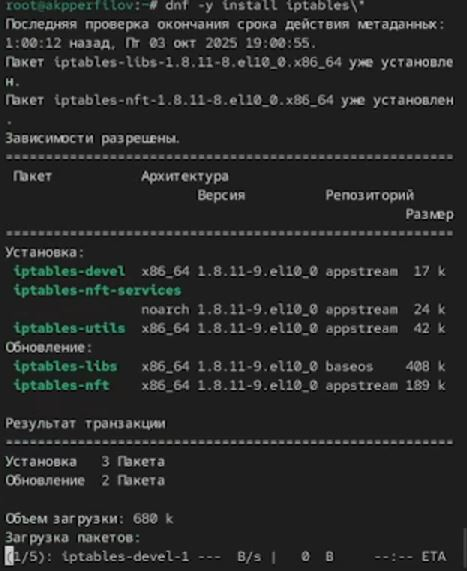
\includegraphics[width=0.71\linewidth,height=\textheight,keepaspectratio]{./home/akpperfilov/work/study/2025-2026/Основы администрирования операционных систем/os2/study_2025-2026_os2/labs/lab05/report/image/12.jpg}

Проверяем статус firewalld и iptables:

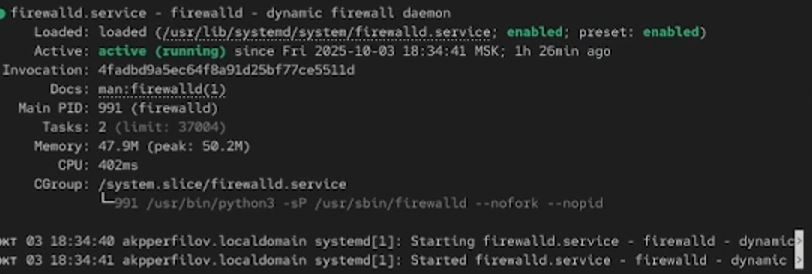
\includegraphics[width=0.71\linewidth,height=\textheight,keepaspectratio]{./home/akpperfilov/work/study/2025-2026/Основы администрирования операционных систем/os2/study_2025-2026_os2/labs/lab05/report/image/13.jpg}

запускаем firewalld и iptables

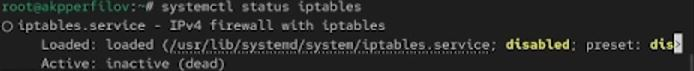
\includegraphics[width=0.71\linewidth,height=\textheight,keepaspectratio]{./home/akpperfilov/work/study/2025-2026/Основы администрирования операционных систем/os2/study_2025-2026_os2/labs/lab05/report/image/14.jpg}

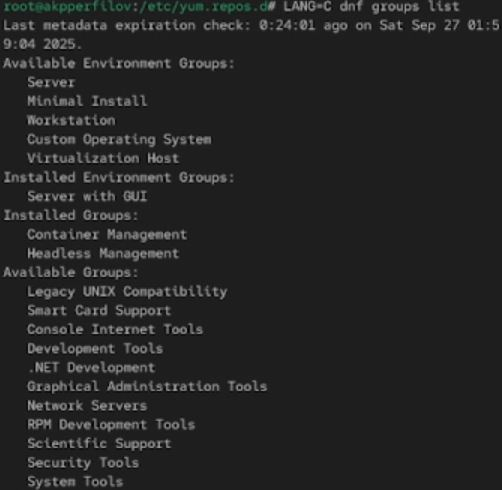
\includegraphics[width=0.71\linewidth,height=\textheight,keepaspectratio]{./home/akpperfilov/work/study/2025-2026/Основы администрирования операционных систем/os2/study_2025-2026_os2/labs/lab05/report/image/15.jpg}

Вводим команду cat /usr/lib/systemd/system/firewalld.service

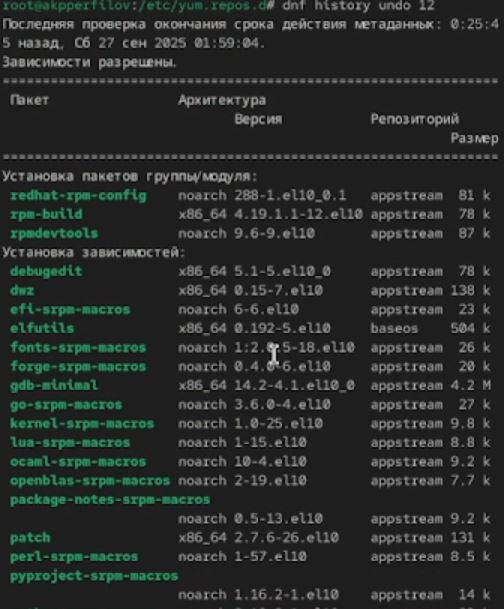
\includegraphics[width=0.71\linewidth,height=\textheight,keepaspectratio]{./home/akpperfilov/work/study/2025-2026/Основы администрирования операционных систем/os2/study_2025-2026_os2/labs/lab05/report/image/17.jpg}

Вводим команду cat /usr/lib/systemd/system/iptables.service

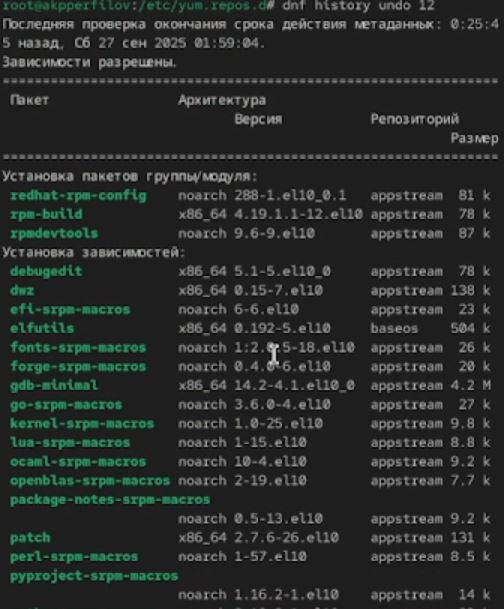
\includegraphics[width=0.71\linewidth,height=\textheight,keepaspectratio]{./home/akpperfilov/work/study/2025-2026/Основы администрирования операционных систем/os2/study_2025-2026_os2/labs/lab05/report/image/17.jpg}

Выгружаем службу iptables

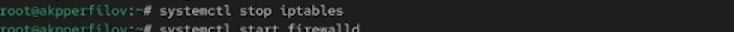
\includegraphics[width=0.71\linewidth,height=\textheight,keepaspectratio]{./home/akpperfilov/work/study/2025-2026/Основы администрирования операционных систем/os2/study_2025-2026_os2/labs/lab05/report/image/18.jpg}

Загружаем службу firewalld

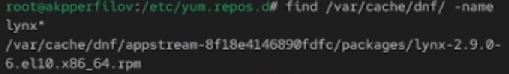
\includegraphics[width=0.71\linewidth,height=\textheight,keepaspectratio]{./home/akpperfilov/work/study/2025-2026/Основы администрирования операционных систем/os2/study_2025-2026_os2/labs/lab05/report/image/19.jpg}

Блокируем запуск iptables

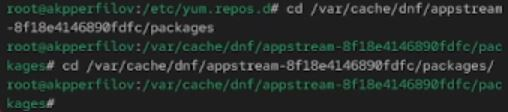
\includegraphics[width=0.71\linewidth,height=\textheight,keepaspectratio]{./home/akpperfilov/work/study/2025-2026/Основы администрирования операционных систем/os2/study_2025-2026_os2/labs/lab05/report/image/20.jpg}

Попробуем запустить iptables:

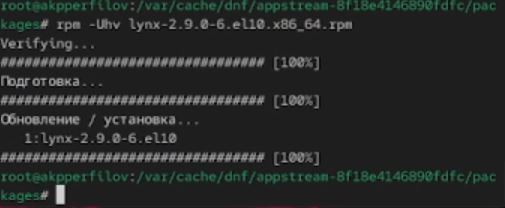
\includegraphics[width=0.71\linewidth,height=\textheight,keepaspectratio]{./home/akpperfilov/work/study/2025-2026/Основы администрирования операционных систем/os2/study_2025-2026_os2/labs/lab05/report/image/21.jpg}

добавляем iptables в автозапуск:

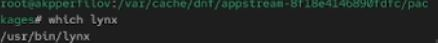
\includegraphics[width=0.71\linewidth,height=\textheight,keepaspectratio]{./home/akpperfilov/work/study/2025-2026/Основы администрирования операционных систем/os2/study_2025-2026_os2/labs/lab05/report/image/22.jpg}

\chapter{Изолируемые
цели}\label{ux438ux437ux43eux43bux438ux440ux443ux435ux43cux44bux435-ux446ux435ux43bux438}

Входим в уч запись root и преходим в каталог systemd

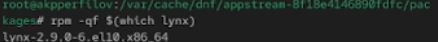
\includegraphics[width=0.71\linewidth,height=\textheight,keepaspectratio]{./home/akpperfilov/work/study/2025-2026/Основы администрирования операционных систем/os2/study_2025-2026_os2/labs/lab05/report/image/23.jpg}

Вводим команду grep isolate *.target

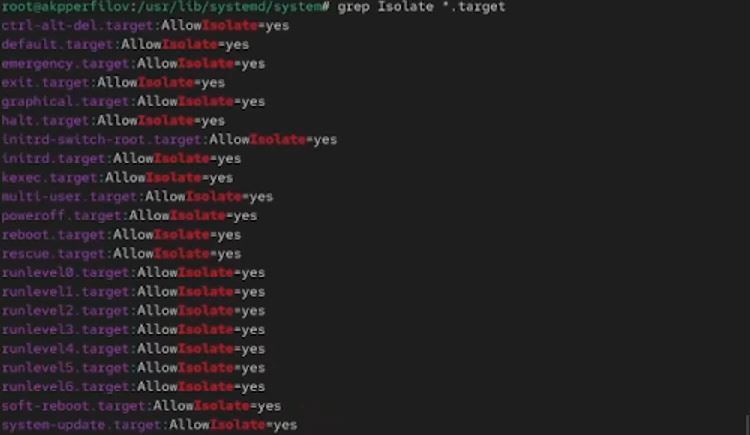
\includegraphics[width=0.71\linewidth,height=\textheight,keepaspectratio]{./home/akpperfilov/work/study/2025-2026/Основы администрирования операционных систем/os2/study_2025-2026_os2/labs/lab05/report/image/24.jpg}

Переключите операционную систему в режим восстановления

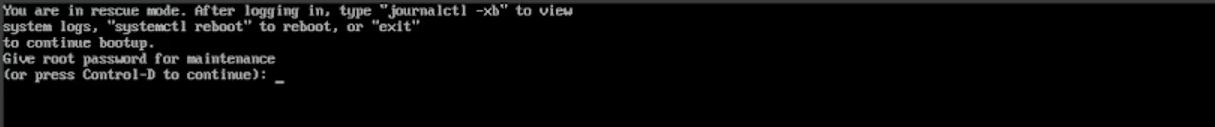
\includegraphics[width=0.71\linewidth,height=\textheight,keepaspectratio]{./home/akpperfilov/work/study/2025-2026/Основы администрирования операционных систем/os2/study_2025-2026_os2/labs/lab05/report/image/25.jpg}

\chapter{Цель по
умолчанию}\label{ux446ux435ux43bux44c-ux43fux43e-ux443ux43cux43eux43bux447ux430ux43dux438ux44e}

Входим в уч запись root и вводим команду systemctl get-default

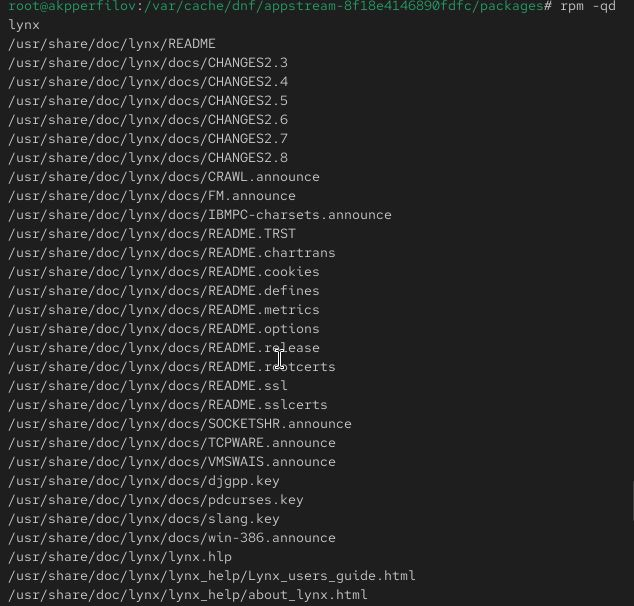
\includegraphics[width=0.71\linewidth,height=\textheight,keepaspectratio]{./home/akpperfilov/work/study/2025-2026/Основы администрирования операционных систем/os2/study_2025-2026_os2/labs/lab05/report/image/26.jpg}

Для установки цели по умолчанию используем systemctl set-default

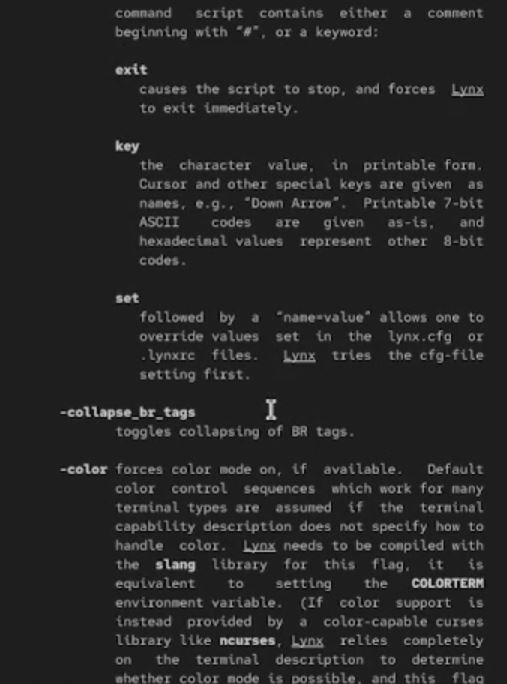
\includegraphics[width=0.71\linewidth,height=\textheight,keepaspectratio]{./home/akpperfilov/work/study/2025-2026/Основы администрирования операционных систем/os2/study_2025-2026_os2/labs/lab05/report/image/27.jpg}

Для запуска по умолчанию текстового режима вводим systemctl set-default
multi-user.target

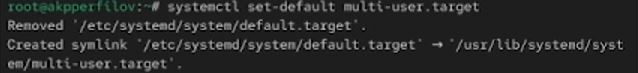
\includegraphics[width=0.71\linewidth,height=\textheight,keepaspectratio]{./home/akpperfilov/work/study/2025-2026/Основы администрирования операционных систем/os2/study_2025-2026_os2/labs/lab05/report/image/28.jpg}

Перезапускаем систему командой reboot

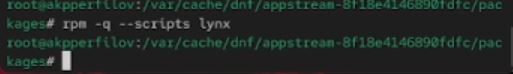
\includegraphics[width=0.71\linewidth,height=\textheight,keepaspectratio]{./home/akpperfilov/work/study/2025-2026/Основы администрирования операционных систем/os2/study_2025-2026_os2/labs/lab05/report/image/29.jpg}

Перезагружаем систему командой reboot

\chapter{Вывод:}\label{ux432ux44bux432ux43eux434}

В ходе работы приобретены умения по работе с управлением системными
службами операционной системы посредством systemd


\printbibliography



\end{document}
